\documentclass[10pt,twocolumn]{article}

\usepackage{geometry}
\geometry{
	a4paper,
	left=1cm,
	top=1cm,
	right=1cm,
	bottom=1cm,
}
\usepackage{color}
\usepackage[toc,page]{appendix}
\usepackage{authblk}
\usepackage{amsmath}
\usepackage{url}
\usepackage{graphicx}
\usepackage{float}
\usepackage{listings}

\definecolor{mygray}{rgb}{0.4,0.4,0.4}
\definecolor{commentscolor}{rgb}{0.6,0.6,0.6}

\lstdefinestyle{cStyle}{
	captionpos=t,
	numbers=left,
	% xleftmargin=8pt,
	numberstyle=\color{mygray}\ttfamily\small,
	numbersep=8pt,
	language=c,
	keywordstyle=\color{blue}\small,
	stringstyle=\color{red}\small,
	commentstyle=\color{commentscolor}\small,
	basicstyle=\ttfamily\small,
	showstringspaces=false,
	breaklines,
	escapechar=|,
	columns=fullflexible,
}

\pagenumbering{gobble}

\begin{document}

\title{\vspace{-1.5cm}Bubble Sort using Domain Decomposition with MPI}
\author[]{Claudio Scheer, Gabriell Araujo}
\date{}

\maketitle


\section*{General Setup}

We ran our \textit{batch job} on two nodes (2x12 cores, 2x24 when considering hyper-threading) in the Cerrado cluster. All experiments were executed three times and then the average execution time and the standard deviation were calculated. Efficiency and speedup were based on the execution time reported by the sequential execution of the bubble sort algorithm.

For the implementation using MPI, we used the domain decomposition philosophy. In short, each process sorts $1/n$ of the vector using the bubble sort algorithm and shares its lowest values with the left neighbor. The piece of the vector shared is interleaved with the vector held by the left neighbor, and the same process is repeated until the vector is sorted. In this report, we discuss three optimization that we perform in this workflow.

\begin{figure}[ht]
	\centering
	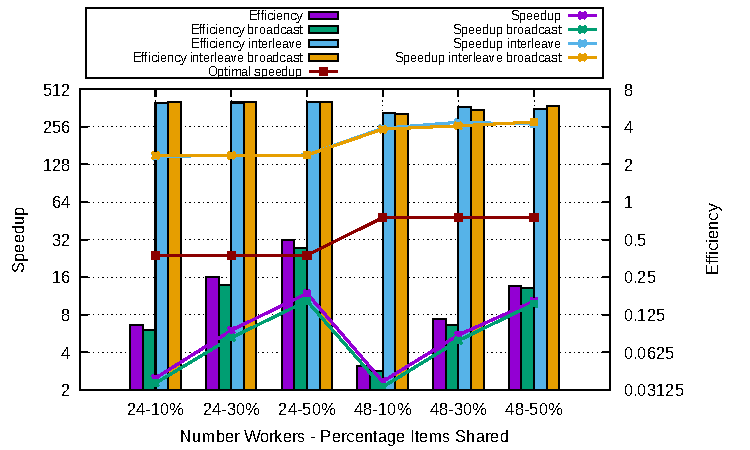
\includegraphics[width=0.45\textwidth]{../logs/scripts/bubble-sort-speedup-efficiency.pdf}
	\caption{Speedup x Efficiency}
	\label{fig:bubble-sort-speedup-efficiency}
\end{figure}


\section*{Bubble Sort without optimizations}

The bubble sort problem addressed here consists of sorting one vector with 1000032 integers. This vector is divided among the processes. Therefore, each process have $n/processes$ integers. As we are sorting a vector in descending order, each process can generate its own vector, without the need to create the entire vector and share it between the processes.

The first phase of the bubble sort algorithm using domain decomposition structure is the application of the bubble sort algorithm over the part of the vector held by each process. After that, each processes communicates with all other processes to test whether they are sorted or not with their neighboring processes. Otherwise, the processes send their lowest numbers to the process on left and receive the highest values from the process on the right. This steps is repeated until the vector is sorted.

According to the results seen in Figure~\ref{fig:bubble-sort-speedup-efficiency}, the speedup of this implementation is deeply related to the percentage of numbers that are shared between the processes. It is important to note that we cannot shared more than 50\% of the vector between processes, since processes other than $0$ and $processes - 1$ will send and receive numbers from the left and right.


\section*{Broadcast optimization}

The first optimization was to reduce the amount of broadcast messages sent by processes to check whether they are all sorted or not when compared with the other processes. Therefore, as soon as a broadcast message returns that a process is not sorted in relation to the left neighbor, we stop sending and receiving broadcast messages.

As shown in Figure~\ref{fig:bubble-sort-speedup-efficiency}, the results using this optimization, compared to results without optimization, were in the range of the standard deviation. Even when the percentage of numbers shared between the processes were higher, which results in faster convergence, the reduction in broadcast messages was not significant. When using up to 264 processes, broadcast messages have an impact of about $\approx$ 66\%, but we can still see that broadcast messages are not the main bottleneck.


\section*{Interleave instead of bubble sort}

The second optimization was focused on reducing the use of the bubble sort algorithm as much as possible, since this algorithm has a time complexity of $O(n^2)$. Thus, as we can interleave the vector with the part of the vector shared between the processes, it is possible to execute the bubble sort algorithm only once in each process. To use interleaving instead of bubble sort, we first interleave the vector with the percentage of numbers received from right, ignoring the percentage of numbers received from the left. Finally, we interleave the ignored part with the entire vector. It is not possible to call only once the interleave method, as we can end up with three vector pieces in a single process.

This optimization lead to a speedup higher than the optimal speedup. As the interleave algorithm has a linear time complexity, the percentage of items shared between the processes does not have a high impact on speedup or efficiency when using all physical cores or hyper-threading.


\section*{Broadcast and interleave}

We also tested using the two optimizations discussed above at the same time. The results showed that this can lead to almost the same results as using just the interleaving optimization. However, when using more process than hyper-threading limit, the results shows that sharing a higher percentage of numbers is better. Despite this, there is a loss of efficiency and, at some point, a lost of speedup. We believe that this is due to the number of broadcast messages that must be used to synchronize all of these processes.


\section*{Discussion}

Finally, the broadcast messages, even when widely required, have no significant impact on the domain decomposition performance with MPI. The main bottleneck in this process is the bubble sort algorithm.

Comparing the domain decomposition, with its better optimization, with the divide and conquer approach shows that divide and conquer has a much better speedup and efficiency when using more processes than hyper-threading.


\onecolumn

\section*{Bubble Sort Source Code}

\lstinputlisting[caption=Dataset generator,style=cStyle]{../bubble-sort/dataset-generator.h}
\lstinputlisting[caption=Bubble Sort Sequential,label=lst:bubble-sort-sequential,style=cStyle]{../bubble-sort/sort-seq.c}
\lstinputlisting[caption=Bubble Sort MPI,label=lst:bubble-sort-mpi,style=cStyle]{../bubble-sort/sort-mpi.c}

\end{document}
